\chapter{p 区（二）：氧、卤素与稀有气体}\label{ch:b1:p-block-16-18}

硫酸的年产量高于任何其他化学品：它
用于溶解磷矿以制造化肥，浸出铜矿石与铀矿石，
精炼石油、配制汽车电池的电解液，一个世纪以来，硫酸的产量
曾是衡量一国工业水平的粗略标尺。其
硫如今大多来自天然气与石油的净化，仍有一些
由人力从火山口中搬出。硫位于第 16 族，处于氧的正下方；
第 17 族的\omterm{def:b1:p-block-16-18:halogen}{卤素}与第 18 族的稀有气体，共同构成
p 区。本章从氧和硫的单质出发，
一直讨论到硫酸；用\omterm{def:b1:nernst:electrode-potential}{标准电极电势}比较\omterm{def:b1:p-block-16-18:halogen}{卤素}作为\omterm{def:b1:nernst:couple}{氧化剂}的强弱，
最后讲述看似惰性的稀有气体确实能够形成的化合物。

\begin{recall}
\omterm{def:b1:lewis-resonance-vsepr:lewis}{路易斯结构}、扩展八隅体及\omterm{def:b1:lewis-resonance-vsepr:vsepr}{价层电子对互斥模型}所得的构型（见\cref{ch:b1:lewis-resonance-vsepr}）；
\omterm{def:b1:nernst:electrode-potential}{标准电极电势}（见\cref{ch:b1:nernst}）；氯的\omterm{def:b1:e-ph-diagrams:disproportionation}{歧化}
及氯的电势–pH 图
（见\cref{ch:b1:e-ph-diagrams}）；催化（见\cref{ch:b1:elementary-steps}）。
第 1 册（十年级）把\omterm{def:b1:p-block-16-18:halogen}{卤素}与稀有气体
归为若干族。
\end{recall}

\begin{omfigure}
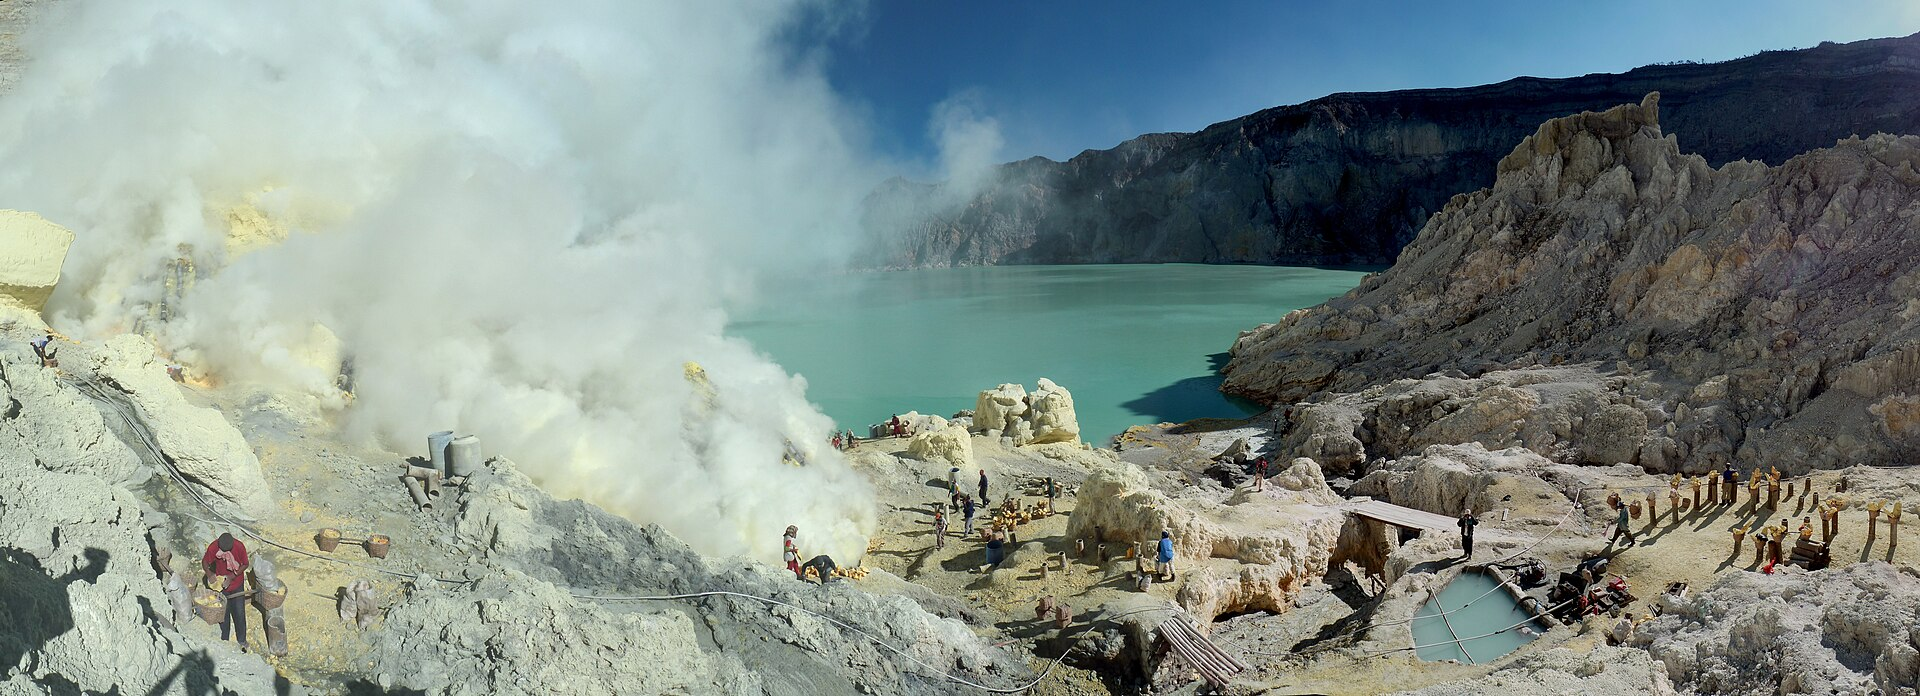
\includegraphics[width=0.78\linewidth]{images/book2/kawah-ijen.jpg}

{\small 印度尼西亚伊真火山口的采硫：
火山气体在管道周围凝结出黄色的硫，矿工
用篮子搬出（照片：Sémhur，CC BY-SA 4.0，维基共享资源）。}
\end{omfigure}

\section{氧、臭氧与过氧化物}

\begin{definition}[氧族元素]\label{def:b1:p-block-16-18:chalcogen}
\emph{氧族元素}\index{氧族元素}是第 16 族元素
（O、S、Se、Te、Po），\omterm{def:b1:quantum-numbers:configuration}{价电子}数为 6，构型为 \textit{ns}$^2$\textit{np}$^4$。
它们形成的化合物中，\omterm{def:b1:nernst:oxidation-number}{氧化数}从 $-$II（氧化物、硫化物）
到 $+$VI（硫酸盐），较高的\omterm{def:b1:nernst:oxidation-number}{氧化数}仅见于硫及其以下的元素。
\end{definition}

氧以氧气 \ce{O2} 与臭氧 \ce{O3} 两种形式存在，其中臭氧为折线形分子，
具有两种\omterm{def:b1:lewis-resonance-vsepr:resonance}{共振结构}（见\cref{ch:b1:lewis-resonance-vsepr}）。臭氧
是比氧气更强的\omterm{def:b1:nernst:couple}{氧化剂}：$E^\circ(\ce{O3}/\ce{O2}) = 2.07$~V
与 1.23~V 的 \ce{O2}/\ce{H2O} 相比。在高层大气中它吸收
紫外线；在近地面，它是污染物。过氧化氢，
含 \ce{O-O} 键，氧的\omterm{def:b1:nernst:oxidation-number}{氧化数}为 $-$I，既是\omterm{def:b1:nernst:couple}{氧化剂}，又是\omterm{def:b1:nernst:couple}{还原剂}，
并会缓慢发生\omterm{def:b1:e-ph-diagrams:disproportionation}{歧化}（见\cref{exo:b1:nernst:12}）。
% ledger: dfg:O3_g (E0 computed in figdata/bachelor-1/standard-potentials.py)

\begin{example}[氧的氧化数]
氧的\omterm{def:b1:periodicity:electronegativity}{电负性}仅次于氟，其\omterm{def:b1:nernst:oxidation-number}{氧化数}在
几乎所有化合物中为 $-$II：水、氧化物、氢氧化物、硫酸盐。
例外情况由如下规则决定：共用电子归\omterm{def:b1:periodicity:electronegativity}{电负性}较大的一方，
若两原子相同，则共用电子在两者之间平分。在
过氧化氢 \ce{H2O2}（H--O--O--H）中，每个氧原子取得其
\ce{O-H} 键的电子，而 \ce{O-O} 键的电子对由两者共用：$-$I。
在超氧化钾 \ce{KO2} 中，离子 \ce{O2-} 的一个电荷由两个原子分摊，
平均为 $-\frac12$。在二氟化氧 \ce{OF2} 中，氟夺得两个键的电子，
氧的\omterm{def:b1:nernst:oxidation-number}{氧化数}为 $+$II。在 \ce{O2} 与 \ce{O3} 中其\omterm{def:b1:nernst:oxidation-number}{氧化数}为 0。只有
$-$II 态对水稳定；过氧化物与超氧化物
是\omterm{def:b1:nernst:couple}{氧化剂}，\ce{OF2} 则是氟化剂。
\end{example}

\section{硫与硫酸}

与氧不同，硫能形成由单键 \ce{S-S} 组成的环和链：
普通硫由 \ce{S8} 环构成。硫燃烧生成二氧化硫，
为折线形分子（O--S--O 键角 \ang{119.5}），可进一步被氧化
为三氧化硫，呈平面三角形。二者都是\omterm{def:b1:s-block:oxide-character}{酸性氧化物}：\ce{SO2}
生成亚硫酸（$\mathrm{p}K_a$ 为 1.77 和 7.22），\ce{SO3} 生成
硫酸。
% ledger: geo:SO2.aOSO, dfg:SO2_g, dfg:SO3_g

\begin{proposition}[接触法的步骤]\label{prop:b1:p-block-16-18:contact-steps}
硫酸由硫分四步制得：
（1）\ce{S + O2 -> SO2}；（2）\ce{2SO2 + O2 <=> 2SO3}，以五氧化二钒
为\omterm{def:b1:elementary-steps:catalyst}{催化剂}；（3）\ce{SO3 + H2SO4 -> H2S2O7}（发烟硫酸），三氧化硫
被浓硫酸吸收；（4）\ce{H2S2O7 + H2O -> 2H2SO4}。总反应为
\ce{2S + 3O2 + 2H2O -> 2H2SO4}。
\end{proposition}

\begin{proof}
各步均已配平。将 $2\times(1)$、(2)、$2\times(3)$ 与
$2\times(4)$ 相加，\ce{SO2}、\ce{SO3} 与 \ce{H2S2O7} 相消，第 3 步消耗的两个
\ce{H2SO4} 在第 4 步中再生，于是得到
\ce{2S + 3O2 + 2H2O -> 2H2SO4}。第 2 步在室温下热力学上非常有利
（\qty{25}{\celsius} 时 $K = 10^{24.8}$，由
生成吉布斯自由能算得），但速率极慢：\omterm{def:b1:elementary-steps:catalyst}{催化剂}仅在加热时有活性，
正是\omterm{def:b1:elementary-steps:catalyst}{催化剂}使反应得以进行；速率与转化率之间的折中
在本科二年级分册中研究。\ce{SO3} 不能直接被水吸收，
因为它与水蒸气反应，会生成细小的
酸雾滴，它们穿过吸收塔。
\end{proof}
% ledger: dfg:SO2_g, dfg:SO3_g

\begin{omfigure}
\begin{tikzpicture}[font=\small, >={Stealth}, box/.style={draw, rounded corners, fill=omDef!8, align=center, minimum height=1.0cm}]
  \node[box] (b) at (0,0) {硫燃烧炉 \\\ce{S + O2 -> SO2}};
  \node[box] (c) at (4.4,0) {转换器，\ce{V2O5}\\催化剂床层};
  \node[box] (a) at (8.8,0) {吸收塔 \\\ce{SO3} 吸入 \ce{H2SO4}};
  \node[box] (d) at (8.8,-2.2) {稀释 \\\ce{H2S2O7 + H2O}};
  \draw[<-, thick] (b.west) -- ++(-0.8,0) node[left] {空气、S};
  \draw[->, thick] (b) -- node[above] {\ce{SO2}} (c);
  \draw[->, thick] (c) -- node[above] {\ce{SO3}} (a);
  \draw[->, thick] (a) -- node[right] {发烟硫酸} (d);
  \draw[->, thick] (d.west) -- ++(-1.2,0) node[left] {\ce{H2SO4}};
  \draw[->, thick] (d.east) -- ++(0.6,0) |- node[pos=0.25, right] {部分返回} (a.east);
\end{tikzpicture}

{\small 接触法：燃烧硫，催化氧化
\ce{SO2}，\ce{SO3} 在浓硫酸中的吸收，以及
发烟硫酸的稀释。部分酸被返回吸收塔。}
\end{omfigure}

\begin{proposition}[硫酸的强度]\label{prop:b1:p-block-16-18:sulfuric-strength}
在水中，硫酸的第一步电离是强的（完全电离），第二步是弱的：
$\mathrm{p}K_a(\ce{HSO4-}/\ce{SO4^2-}) = 1.99$。
\qty{0.010}{mol/L} 溶液的 pH 因此不在 1.70（两个质子）处，也不在
2.00（一个质子）处，而介于两者之间。
\end{proposition}

\begin{proof}
\ce{H2SO4} 中硫上连有两个不含氢的氧，是一种
酸性强于 \ce{H3O+} 的\omterm{def:b1:p-block-13-15:oxoacid}{含氧酸}，在水中被拉平（见\cref{ch:b1:predominant-reaction}）。
\ce{HSO4-} 已带负电，更牢固地持有质子：其 $\mathrm{p}K_a$，
由生成吉布斯自由能算得为 1.99。当 $C = 0.010$ 时：
$[\ce{H3O+}] = C + x$，$[\ce{HSO4-}] = C - x$，$[\ce{SO4^2-}] = x$，其中
$x(C + x)/(C - x) = 10^{-1.99}$；解得 $x = \qty{4.2e-3}{mol/L}$，且
$\mathrm{pH} = -\log(0.0142) = 1.85$。
\end{proof}
% ledger: dfg:HSO4-_ao, dfg:SO42-_ao

浓硫酸也是一种强\omterm{def:b1:alcohol-activation:dehydration}{脱水}剂（能使糖炭化，
夺取糖中水的组成元素），加热时还是一种\omterm{def:b1:nernst:couple}{氧化剂}。稀释时
放出大量热：酸应始终倒入水中，绝不能
反过来操作。2025 年全球约 8400 万吨硫，其中大部分
由天然气和炼油气流中的硫化氢回收而得，
并且大部分最终制成硫酸。
% ledger: usgs:S-world-2025

\begin{method}[通过接触法的质量衡算]\label{met:b1:p-block-16-18:contact-balance}
\begin{enumerate}
  \item 使用总方程式：每个 S 原子生成一个 \ce{H2SO4}。
  \item 修正第 2 步的转化（被氧化的 \ce{SO2}
        所占比例），以及吸收中的损失。
  \item 对于空气：计算所需 \ce{O2}（每个 S 需 1.5 个），
        再除以其在空气中的体积分数。
\end{enumerate}
\end{method}

\begin{example}[每天燃烧一千吨硫的工厂]
一座工厂每天燃烧 \qty{1000}{t} 硫，转化 \qty{99.0}{\percent}
的 \ce{SO2}，吸收 \qty{99.9}{\percent} 的 \ce{SO3}。于是
$n(\ce{S}) = \num{1000e6}/32.1 = \qty{3.12e7}{mol}$，且
$n(\ce{H2SO4}) = \num{3.12e7} \times 0.990 \times 0.999
= \qty{3.08e7}{mol}$，即 $\num{3.08e7} \times \qty{98.1}{g}
= \qty{3020}{t}$ 的酸（每天）。未转化的 \qty{1.0}{\percent} 以
\ce{SO2} 形式排出：\qty{3.1e5}{mol}，即每天 \qty{20}{t}，须从
尾气中除去。所需氧气为 $1.5 \times \num{3.12e7} =
\qty{4.67e7}{mol}$；空气中 \ce{O2} 占 \qty{21}{\percent}，所需空气量为
\qty{2.23e8}{mol}，或每天 $V = nRT/p = \qty{5.5e6}{m^3}$，在
\qty{25}{\celsius} 与 \qty{1}{bar} 下，未计入工厂
实际鼓入的过量空气。
\end{example}
% ledger: air:O2

\section{卤素}

\begin{definition}[卤素]\label{def:b1:p-block-16-18:halogen}
\emph{卤素}\index{卤素}是第 17 族元素（F、Cl、
Br、I、At），具有七个\omterm{def:b1:quantum-numbers:configuration}{价电子} \textit{ns}$^2$\textit{np}$^5$。
它们以双原子分子 \ce{X2} 存在，并形成卤离子 \ce{X-}。
\end{definition}

\begin{omfigure}
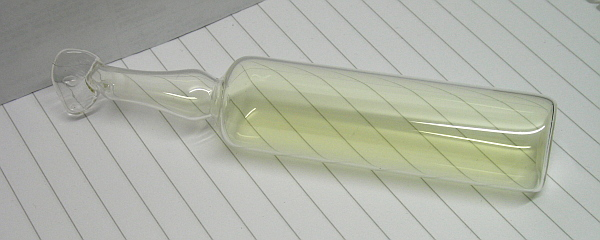
\includegraphics[height=2.9cm]{images/book2/chlorine.jpg}\hspace{0.5em}%
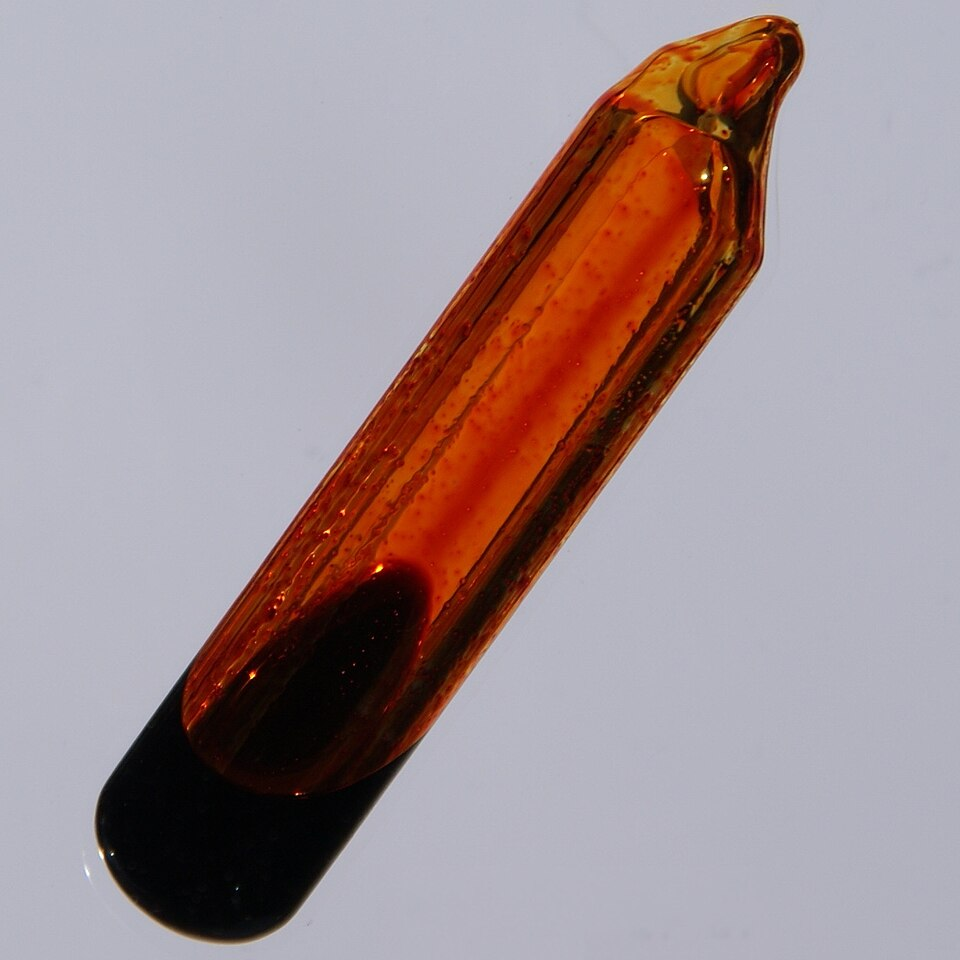
\includegraphics[height=2.9cm]{images/book2/bromine.jpg}\hspace{0.5em}%
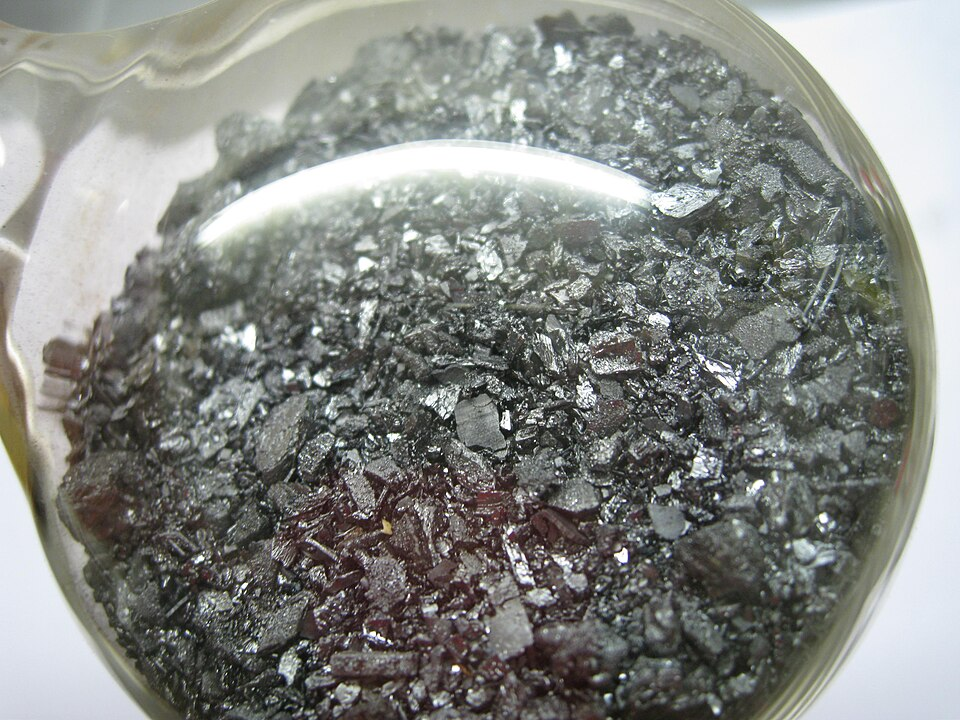
\includegraphics[height=2.9cm]{images/book2/iodine.jpg}

{\small 氯气，淡黄绿色气体（照片：W. Oelen，CC BY-SA 3.0）；
溴，深红色液体，带橙色蒸气（照片：Jurii，CC BY 3.0）；碘，
灰黑色\omterm{def:b1:crystals-metals:crystal}{晶体}，具有金属光泽（照片：Dnn87，CC BY 3.0）。氯与
溴密封于玻璃安瓿中。图片均来自维基共享资源。}
\end{omfigure}

\begin{proposition}[卤素的氧化能力]\label{prop:b1:p-block-16-18:halogen-oxidising-order}
\omterm{def:b1:p-block-16-18:halogen}{卤素}是\omterm{def:b1:nernst:couple}{氧化剂}，其氧化能力沿族向下减弱：
$E^\circ(\ce{F2}/\ce{F-}) = 2.89$~V，\ce{Cl2}/\ce{Cl-} 1.36~V，
\ce{Br2}/\ce{Br-} 1.08~V，\ce{I2}/\ce{I-} 0.53~V。每种\omterm{def:b1:p-block-16-18:halogen}{卤素}都能氧化
同族中位于其下方的卤离子。
\end{proposition}

\begin{proof}
这些数值由卤离子的生成吉布斯自由能算得
（见\cref{ch:b1:nernst}）。由 γ 规则，\ce{X2} 氧化 \ce{Y-} 的条件是
\ce{X2}/\ce{X-} 电对位于 \ce{Y2}/\ce{Y-} 之上：例如
\ce{Cl2 + 2Br- -> 2Cl- + Br2}，$\log K = 2(1.36 - 1.08)/0.059 = 9.5$。
沿族向下，原子增大，其\omterm{def:b1:periodicity:electron-affinity}{电子亲和能}
及较小卤离子的水合作用均减弱，电势随之下降。
\end{proof}
% ledger: dfg:F-_ao, dfg:Cl-_ao, dfg:Br-_ao, dfg:I-_ao

\begin{omfigure}
\begin{tikzpicture}
\begin{axis}[
  ybar, width=0.62\linewidth, height=5.0cm, ymin=0, ymax=3.3,
  symbolic x coords={F,Cl,Br,I}, xtick=data,
  xticklabels={\ce{F2}/\ce{F-}, \ce{Cl2}/\ce{Cl-}, \ce{Br2}/\ce{Br-}, \ce{I2}/\ce{I-}},
  ylabel={$E^\circ$ (V)}, bar width=16pt, nodes near coords,
  every node near coord/.append style={font=\scriptsize},
  tick label style={font=\small}, label style={font=\small}, enlarge x limits=0.2]
\addplot[fill=omThm!40, draw=omThm] coordinates {(F,2.89) (Cl,1.36) (Br,1.08) (I,0.53)};
\end{axis}
\end{tikzpicture}

{\small \omterm{def:b1:p-block-16-18:halogen}{卤素}–卤离子电对的\omterm{def:b1:nernst:electrode-potential}{标准电极电势}，在
\qty{25}{\celsius} 下，由表列吉布斯自由能算得：
氧化能力沿族向下稳定减弱。}
\end{omfigure}

卤化氢在水中都是酸，但 \ce{HF} 为\omterm{def:b1:predominant-reaction:strong-acid}{弱酸}，
（$\mathrm{p}K_a$ 3.16），而 \ce{HCl}、\ce{HBr} 和 \ce{HI} 为\omterm{def:b1:predominant-reaction:strong-acid}{强酸}：
\ce{H-F} 键很强，较小的氟离子被
强\omterm{def:b1:intermolecular-forces-solvents:hbond}{氢键}束缚。氟是\omterm{def:b1:periodicity:electronegativity}{电负性}最大的元素，也是
表中最强的\omterm{def:b1:nernst:couple}{氧化剂}，只能通过电解制得。
氯的\omterm{def:b1:p-block-13-15:oxoacid}{含氧酸}——次氯酸 \ce{HClO}、氯酸 \ce{HClO3}、
高氯酸 \ce{HClO4}——随不含氢的氧原子数目增加而变强，
这与所有\omterm{def:b1:p-block-13-15:oxoacid}{含氧酸}的规律一致（见\cref{def:b1:p-block-13-15:oxoacid}）；它们
与氯离子和氯之间的相互关系，已在
\cref{ch:b1:e-ph-diagrams}中作出了图示。
% ledger: dfg:HF_ao, dfg:F-_ao

\begin{omfigure}
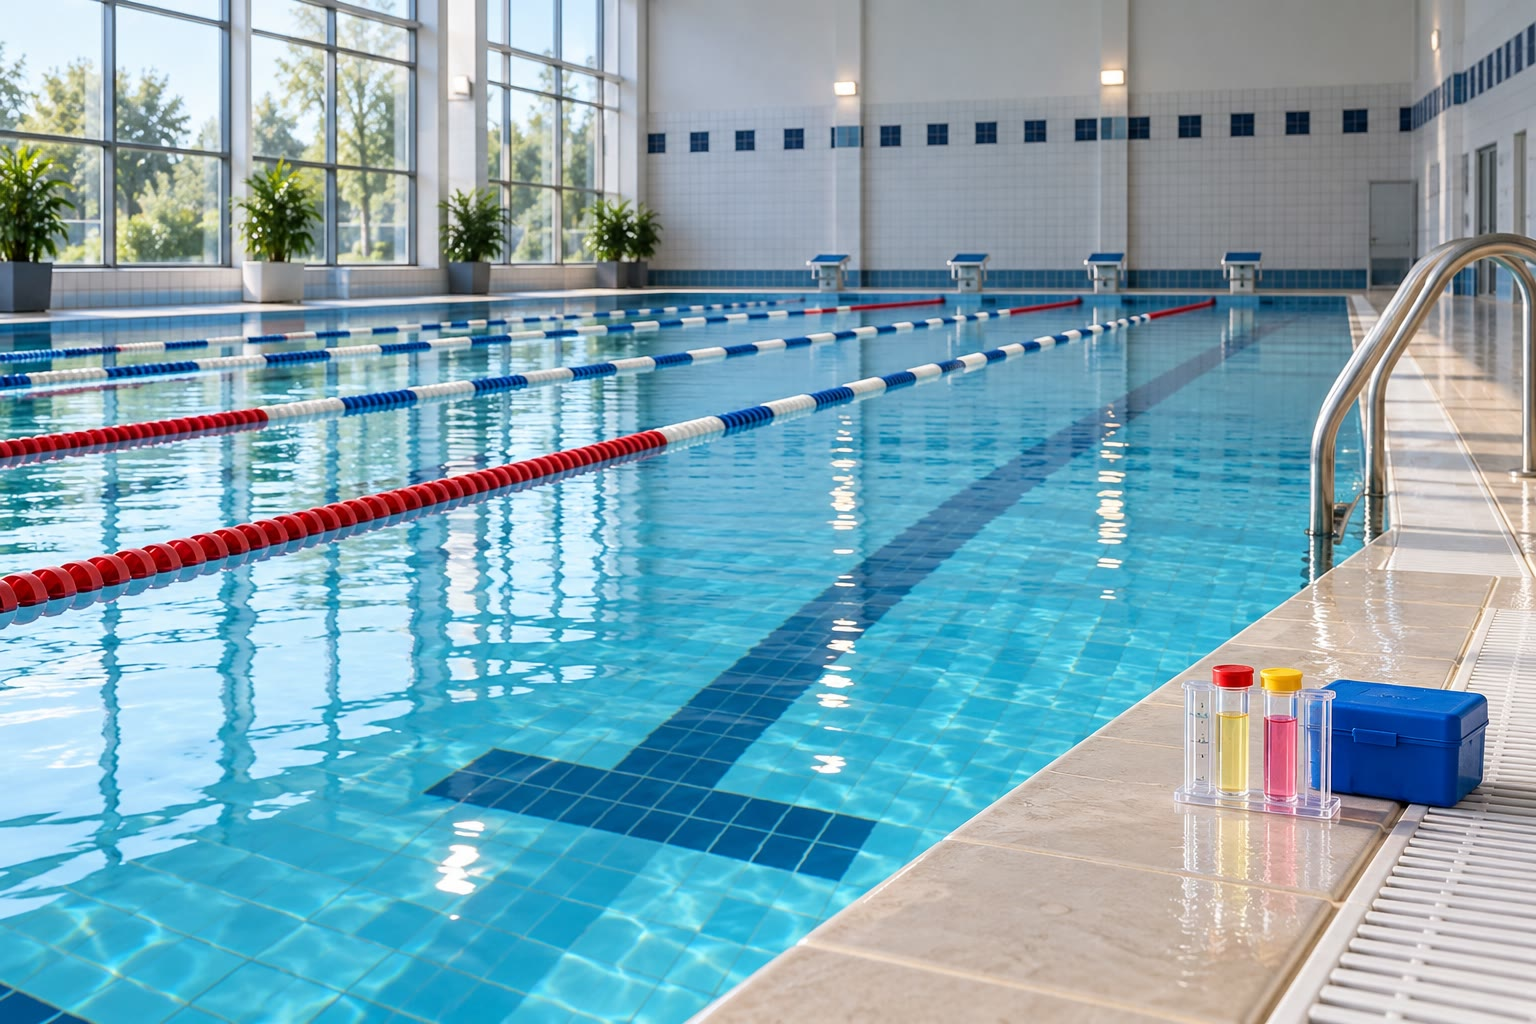
\includegraphics[width=0.55\linewidth]{images/book2/ai/b1-28-swimming-pool.jpg}

{\small 一座公共游泳池及其水质检测工具：溶解为次氯酸的氯，
每天需检测多次。}
\end{omfigure}

\begin{definition}[卤素互化物]\label{def:b1:p-block-16-18:interhalogen}
称\emph{卤素互化物}\index{卤素互化物}为两种不同\omterm{def:b1:p-block-16-18:halogen}{卤素}组成的化合物，
例如 \ce{ICl}、\ce{BrF3}、\ce{ClF3}、\ce{IF7}。
其中原子半径较大、\omterm{def:b1:periodicity:electronegativity}{电负性}较小的\omterm{def:b1:p-block-16-18:halogen}{卤素}为\omterm{def:b1:complexation:complex}{中心原子}，
在 \ce{ClF3} 及更高的化合物中，\omterm{def:b1:complexation:complex}{中心原子}的八隅体被扩展。
\end{definition}

\begin{inthelab}[卤素的操作]
氯有毒，只能在通风橱中少量制备；溴会灼伤皮肤，其蒸气伤害肺部，
使用时须稀释，
并在通风橱中戴手套和护目镜操作，手边备好硫代硫酸钠溶液，
用于处理溢出物
（\ce{4Br2 + S2O3^2- + 5H2O -> 8Br- + 2SO4^2- + 10H+}）。碘是三者中最温和的，
但会染色并升华，应装在密闭的瓶中保存。
\end{inthelab}

\section{稀有气体及其化合物}

稀有气体（He、Ne、Ar、Kr、Xe、Rn）的价\omterm{def:b1:quantum-numbers:orbital}{电子层}已充满，其电离能在各自\omterm{def:b1:periodicity:table}{周期}中最高
（见\cref{ch:b1:periodicity}）。
人们长期认为它们是惰性的，但较重的稀有气体，外层电子束缚较弱，
确实能与\omterm{def:b1:periodicity:electronegativity}{电负性}最大的元素反应：氙可生成
\ce{XeF2}、\ce{XeF4}、\ce{XeF6} 及氧化物。它们的几何构型遵循价层电子对互斥规则，
氙原子上带有\omterm{def:b1:lewis-resonance-vsepr:lewis}{孤电子对}。

\begin{example}[为什么是氙而不是氩]
稀有气体的\omterm{def:b1:periodicity:ionisation-energy}{第一电离能}沿族向下递减：He
24.59、Ne 21.56、Ar 15.76、Kr 14.00、Xe 12.13、Rn 10.75~eV。氧分子的
\omterm{def:b1:periodicity:ionisation-energy}{第一电离能} \ce{O2 -> O2+ + e-} 为 12.07~eV，与氙的几乎相同。
因此，能从 \ce{O2} 夺取一个电子、生成二氧基阳离子 \ce{O2+} 的\omterm{def:b1:nernst:couple}{氧化剂}，
也应能氧化氙，但不能氧化氩，
因为氩对其电子的束缚要紧 3.7~eV。氙确实能与极强的\omterm{def:b1:nernst:couple}{氧化剂}六氟化铂 \ce{PtF6} 反应，
生成总组成为 \ce{XePtF6} 的固体，
也能与氟单质反应，生成下表所列的氟化氙。
氡更易电离，
但放射性太强，难以对其进行大量化学研究。
\end{example}
% ledger: ie:He, ie:Ne, ie:Ar, ie:Kr, ie:Xe, ie:Rn, ie:O2, lit:XePtF6

\begin{omfigure}
\begin{tabular}{llll}
\hline
分子 & \omterm{def:b1:complexation:complex}{中心原子}上的电子对 & 形状 & 实测键角 \\
\hline
\ce{SO2} & 2 个成键电子域 + 1 个\omterm{def:b1:lewis-resonance-vsepr:lewis}{孤电子对} & 角形 & \ang{119.5} \\
\ce{SF6} & 6 个成键电子域 & 八面体形 & \ang{90} \\
\ce{ClF3} & 3 个成键电子域 + 2 个\omterm{def:b1:lewis-resonance-vsepr:lewis}{孤电子对} & T 形 & \ang{87.5} \\
\ce{XeF2} & 2 个成键电子域 + 3 个\omterm{def:b1:lewis-resonance-vsepr:lewis}{孤电子对} & 直线形 & \ang{180} \\
\ce{XeF4} & 4 个成键电子域 + 2 个\omterm{def:b1:lewis-resonance-vsepr:lewis}{孤电子对} & 平面四方形 & \ang{90} \\
\hline
\end{tabular}

\smallskip
{\small 部分带有扩展八隅体或\omterm{def:b1:lewis-resonance-vsepr:lewis}{孤电子对}的 p 区分子的形状
（有实测键角者已列出）。\ce{XeF2} 的\omterm{def:b1:lewis-resonance-vsepr:lewis}{孤电子对}占据三角双锥的
三个平伏位置，
使分子呈直线形。}
% ledger: geo:SO2.aOSO, geo:SF6.aFSF, geo:ClF3.aFClF, geo:XeF2.aFXeF
\end{omfigure}

氩约占空气的百分之一，用于实验室和焊接中保护活泼材料；
氦取自天然气，用于冷却超导磁铁，例如
核磁共振谱仪中的磁铁（见\cref{ch:b1:structure-spectroscopy}）。
% ledger: air:Ar

\section{练习}

\begin{exercise}[$\star$]\label{exo:b1:p-block-16-18:1}
求 \ce{H2S}、\ce{S8}、\ce{SO2}、
\ce{SO3^2-}、\ce{SO4^2-}、\ce{S2O3^2-}（平均值）及 \ce{H2S2O7} 中硫的\omterm{def:b1:nernst:oxidation-number}{氧化数}。
\end{exercise}

\begin{exercise}[$\star$]\label{exo:b1:p-block-16-18:2}
下列反应中哪些能够发生：氯与碘化钾；碘与溴化钠；
溴与氯化钠；氯与溴化钠？
写出能够发生的反应。
\end{exercise}

\begin{exercise}[$\star$]\label{exo:b1:p-block-16-18:3}
画出 \ce{SO2}、\ce{SO3} 和 \ce{O3} 的\omterm{def:b1:lewis-resonance-vsepr:lewis}{路易斯结构}，
及其\omterm{def:b1:lewis-resonance-vsepr:resonance}{共振结构}，并给出它们的形状。
\end{exercise}

\begin{exercise}[$\star$]\label{exo:b1:p-block-16-18:4}
写出 \ce{SO2} 和 \ce{SO3} 分别与水、
与氢氧化钠反应的方程式。
\end{exercise}

\begin{exercise}[$\star\star$]\label{exo:b1:p-block-16-18:5}
计算 \qty{0.10}{mol/L} 氢氟酸的 pH，
并与相同浓度的盐酸比较，解释两者的差异。
\end{exercise}

\begin{exercise}[$\star\star$]\label{exo:b1:p-block-16-18:6}
用\omterm{def:b1:lewis-resonance-vsepr:vsepr}{价层电子对互斥模型}预测 \ce{BrF5}、\ce{IF7}（七个\omterm{def:b1:lewis-resonance-vsepr:lewis}{成键电子对}，
五角双锥）、\ce{ICl4-} 和 \ce{XeO3} 的形状。
\end{exercise}

\begin{exercise}[$\star\star$]\label{exo:b1:p-block-16-18:7}
计算反应 \ce{Cl2 + 2I- -> 2Cl- + I2} 的平衡常数，
并说明氯水为何能使淀粉–碘化钾试纸变蓝。
\end{exercise}

\begin{exercise}[$\star\star$]\label{exo:b1:p-block-16-18:8}
证明臭氧能将碘离子氧化为碘单质，并写出酸性条件下
的反应式。为何可用此反应测定臭氧？
\end{exercise}

\begin{exercise}[$\star\star$]\label{exo:b1:p-block-16-18:9}
浓硫酸能使蔗糖 \ce{C12H22O11} 炭化。写出
\omterm{def:b1:alcohol-activation:dehydration}{脱水}生成碳的反应，并计算由 \qty{10.0}{g} 的
蔗糖可得碳的质量。
\end{exercise}

\begin{exercise}[$\star\star\star$]\label{exo:b1:p-block-16-18:10}
计算 \qty{0.10}{mol/L} 硫酸的 pH，并考虑第二步
电离（$\mathrm{p}K_a = 1.99$）。
第二步电离又使酸度增加了多少？
\end{exercise}

\begin{exercise}[$\star\star\star$]\label{exo:b1:p-block-16-18:11}
利用\omterm{def:b1:nernst:electrode-potential}{电极电势}说明：为何不能用水中任何化学\omterm{def:b1:nernst:couple}{氧化剂}
氧化氟化物来制取氟，以及为何必须电解熔融氟化物
以制取氟，而不能电解其水溶液。
\end{exercise}

\begin{exercise}[$\star\star\star$]\label{exo:b1:p-block-16-18:12}
碘在水中仅微溶，但能以三碘离子 \ce{I3-} 的形式溶于
碘化钾溶液。利用下列物种的吉布斯自由能，
\ce{I2(aq)}（$\Delta_f G^\circ = \qty{16.40}{kJ/mol}$）、\ce{I-}（$-51.57$）
和 \ce{I3-}（$-51.4$），计算反应 \ce{I2 + I- <=> I3-} 的平衡常数。
\end{exercise}

\section{问题：一吨硫}

\begin{problem}[{周末问题——硫的燃烧、二氧化硫的催化
氧化、吸收与发烟硫酸、硫酸的第二步电离，以及
一吨硫所制得硫酸的质量}]
\label{pb:b1:p-block-16-18:1}
某硫酸厂焚烧从天然气中回收的硫。摩尔质量
（\unit{g/mol}）：S 32.1，\ce{O2} 32.0，\ce{SO2} 64.1，\ce{SO3} 80.1，
\ce{H2SO4} 98.1，\ce{H2O} 18.0；空气中 \qty{21}{\percent} 为
\ce{O2}（按体积计）；$\mathrm{p}K_a(\ce{HSO4-}) = 1.99$；$R =
\qty{8.314}{J/(K.mol)}$。

\medskip
\noindent\textbf{第一部分——硫的燃烧。}
\begin{enumerate}
  \item 给出 S、\ce{SO2}、\ce{SO3} 和
        \ce{H2SO4} 中 S 的\omterm{def:b1:nernst:oxidation-number}{氧化数}。
  \item 写出硫的燃烧反应。
  \item 画出 \ce{SO2} 的\omterm{def:b1:lewis-resonance-vsepr:lewis}{路易斯结构}，并预测其形状。
  \item 计算一吨硫中硫的物质的量。
  \item 计算空气的体积（\qty{25}{\celsius}，\qty{1}{bar}），
        仅计燃烧过程。
  \item 为何在进入转化器之前要先将燃烧炉出来的气体冷却？
\end{enumerate}

\medskip
\noindent\textbf{第二部分——催化氧化。}
\begin{enumerate}[resume]
  \item 写出 \ce{SO2} 氧化为 \ce{SO3} 的反应。
  \item 其在 \qty{25}{\celsius} 时的平衡常数约为 $10^{24.8}$，为何仍需
        使用\omterm{def:b1:elementary-steps:catalyst}{催化剂}？
  \item 五氧化二钒的作用是什么？请用
        \cref{ch:b1:elementary-steps}中的语言回答。
  \item 画出 \ce{SO3} 的形状。
  \item 为何要使用过量空气？
  \item 若转化率为
        \qty{99.7}{\percent}，则 \ce{SO2} 损失的比例是多少？
\end{enumerate}

\medskip
\noindent\textbf{第三部分——吸收。}
\begin{enumerate}[resume]
  \item 写出 \ce{SO3} 被硫酸吸收的反应。
  \item 为何 \ce{SO3} 不能直接被水吸收？
  \item 写出发烟硫酸的稀释反应。
  \item 写出该过程的总反应方程式。
  \item 计算每吨硫消耗的水的质量。
  \item 为何必须将酸倒入水中，而绝不能反过来操作？
\end{enumerate}

\medskip
\noindent\textbf{第四部分——硫酸。}
\begin{enumerate}[resume]
  \item 计算 \qty{0.050}{mol/L} 硫酸溶液的 pH，
        并考虑第二步电离。
  \item 计算总\omterm{def:b1:extent-q-and-k:fractional-extent}{产率}为
        \qty{99.5}{\percent} 时可得硫酸的质量。
  \item 2025 年全球约产硫 \qty{84}{Mt}，若
        全部转化，则可得多少质量的硫酸？
  \item 给出一吨硫（完全转化）
        可制得硫酸的质量。
\end{enumerate}
\end{problem}
